\documentclass[19pt,landscape]{article}
\usepackage[landscape]{geometry}
\geometry{a5paper,scale=0.8}
\usepackage{listings}
%\geometry{left=1.5cm,right=1.5cm,top=1.5cm,bottom=0.5cm}
\usepackage{color}
% \usepackage{ulem} % for strikethrough
\usepackage{amsfonts}
\usepackage{Sweave}
\usepackage{bm}
\usepackage{graphicx} 
\usepackage{amsfonts,amsmath,latexsym,amssymb,mathrsfs,amsthm,mathtools}
% \usepackage[british]{babel}
%\usepackage[T1]{fontenc}
%\usepackage{mathptmx}
% \usepackage{times}
\usepackage{datetime2}
\usepackage{filemod}
% \usepackage{fontspec}    %change font 
% \setmainfont{Times New Roman}%fontspec下这个命令设置全局默认字体
\newtheorem{thm}{Theorem}%[section]
\newtheorem{prop}[thm]{Proposition}
\newtheorem{defi}[thm]{Definition}
\newtheorem{lma}[thm]{Lemma}
\newtheorem{cor}[thm]{Corollary}
\newtheorem{exam}[thm]{Example}
\newtheorem{countexam}[thm]{Counterexample}
\newtheorem{rem}[thm]{Remark}
\newtheorem{con}[thm]{Conjecture}
%\bracketfactory{floor}{\lfloor}{\rfloor}
\usepackage{enumerate}
\usepackage{color}
%\usetheme{Copenhagen}
\usepackage[english]{babel}
\usepackage[utf8x]{inputenc}
\newcommand{\law}{\mathscr{L}}
\newcommand{\HH}{\mathscr{H}}
\newcommand{\D}{\mathbb{D}}
\newcommand{\IP}{\mathbb{P}} 
\newcommand{\bone}{{\bf 1}}
\DeclareMathOperator{\E}{\mathbb{E}}
\DeclareMathOperator*{\esssup}{ess\,sup}
\newcommand{\IE}{\E}
\newcommand{\mean}{\E}
\newcommand{\R}{\mathbb{R}}
\newcommand{\N}{\mathbb{N}}
\newcommand{\non}{\nonumber}
\newcommand{\Z}{\mathbb{Z}}
\newcommand{\C}{\mathbb{C}}
%\newcommand{\C}{{\mathds{C}}}
\newcommand{\ci}{{\cal I}}
\newcommand{\cf}{{\cal F}}
\newcommand{\LL}{\textbf{L}}
\DeclareMathOperator{\Var}{\mathrm{Var}}
\DeclareMathOperator{\var}{\mathrm{Var}}
\DeclareMathOperator{\cov}{\mathrm{Cov}}
\DeclareMathOperator{\corr}{\mathrm{Corr}}
\DeclareMathOperator{\bs}{\mathrm{Bias}}
\DeclareMathOperator{\bigo}{\mathrm{O}}
\newcommand{\K}{\textbf{Ker}}
\newcommand{\Id}{\textbf{Id}}
\newcommand{\Pn}{{\rm Pn}}
\newcommand{\dtv}{{d_{\rm TV}}}
\newcommand{\dk}{{d_{\rm K}}}
\newcommand{\dw}{{d_{\rm W}}}
\def\tg{{\tilde g}}
\def\a{{\alpha}}
\def\cn{{\mathcal{N}}}
\def\equald{\stackrel{\mbox{\scriptsize{{\rm d}}}}{=}}
\def\ER{Erd\H{o}s-R\'enyi}
\usepackage{color} 
\definecolor{lightblue}{rgb}{0,0.2,0.5}
\usepackage[colorlinks=true, urlcolor=lightblue,linkcolor=lightblue, citecolor=lightblue]{hyperref}

%%%%%%%%%%%%%%%%%%%%%%%%%%%%%%%%%%

%%% Define bracket commands
\def\given{\mskip 0.5mu plus 0.25mu\vert\mskip 0.5mu plus 0.15mu}
\newcounter{@bracketlevel}
\def\@bracketfactory#1#2#3#4#5#6{
\expandafter\def\csname#1\endcsname##1{%
\addtocounter{@bracketlevel}{1}%
\global\expandafter\let\csname @middummy\alph{@bracketlevel}\endcsname\given%
\global\def\given{\mskip#5\csname#4\endcsname\vert\mskip#6}\csname#4l\endcsname#2##1\csname#4r\endcsname#3%
\global\expandafter\let\expandafter\given\csname @middummy\alph{@bracketlevel}\endcsname
\addtocounter{@bracketlevel}{-1}}%
}
\def\bracketfactory#1#2#3{%
\@bracketfactory{#1}{#2}{#3}{relax}{0.5mu plus 0.25mu}{0.5mu plus 0.15mu}
\@bracketfactory{b#1}{#2}{#3}{big}{1mu plus 0.25mu minus 0.25mu}{0.6mu plus 0.15mu minus 0.15mu}
\@bracketfactory{bb#1}{#2}{#3}{Big}{2.4mu plus 0.8mu minus 0.8mu}{1.8mu plus 0.6mu minus 0.6mu}
\@bracketfactory{bbb#1}{#2}{#3}{bigg}{3.2mu plus 1mu minus 1mu}{2.4mu plus 0.75mu minus 0.75mu}
\@bracketfactory{bbbb#1}{#2}{#3}{Bigg}{4mu plus 1mu minus 1mu}{3mu plus 0.75mu minus 0.75mu}
}


% \title{Nonparametric Regression}
% \author{Qingwei Liu}
% \institute{National University of Singapore}
% \date{\today}

\begin{document}
% \maketitle
%
\setkeys{Gin}{width=0.16\textwidth}
% \begin{titlepage}
% \begin{center}
%     \vfill
% \textbf{\huge ST5207 Nonparametric Regression\\
% Semester 1, AY2024/25}\\[4cm]
% \begin{minipage}{0.4\textwidth}
% \begin{center} \large
% Lecturer:~Qingwei Liu\\
% % Email:liu\_qw@nus.edu.sg\\
% \vskip 6pt
% Department of Statistics and Data Science\\
% \vskip 6pt
% National University of Singapore
% \end{center}
% \end{minipage}%\\[1cm]
% \vfill
% % \includegraphics[width=0.1\textwidth]{./logo}\\[0.5cm]
% \vfill
% \end{center}

% \end{titlepage}
%

\newpage
{\LARGE\centerline{\textbf{Lecture~3:~Kernel Density Estimation}\footnote{Last modified in \filemodprintdate{Lecture3}.}}}
\vskip25pt
\begin{minipage}{.9\textwidth}
    \Large
\begin{itemize}
\item Shortcomings of the Histogram method
\item The native estimator
\item Kernel Functions  
\item The kernel density estimator
\item Theoretical properties 
\item The optimal kernel

\end{itemize}
\end{minipage}
\newpage
{\Large\centerline{\textbf{Shortcomings of Histogram method}}}
\vskip25pt
\begin{minipage}{.9\textwidth}
    \Large
\begin{itemize}
    \item[$\blacktriangleright$] Too restrictive: for every $x$ in the same interval $B_j=[x_0+jh, x_0+(j+1)h)$, histogram assigns the same estimator $\hat{f}_h(x_0+jh)$;
    \item[$\blacktriangleright$] Not continuous: no matter how $f$ looks like;
    \item[$\blacktriangleright$] The convergence rate $O(n^{-2/3})$ of MSE is too slow.  
\end{itemize}
For a continuous density estimator, probably the convergence rate of its MSE could be improved to a better asymptotic order, more close to $O(n^{-1})$.
\end{minipage}



\newpage
{\LARGE\centerline{\textbf{From the native estimator}}}
\vskip25pt
\begin{minipage}{.9\textwidth}
    \Large 
   The native estimator:
   \begin{equation}
    \hat{f}_n(x):=\frac1{2nh}\sum_{i=1}^n\bone_{\{x-h<X_i\le x+h\}}=\frac1{nh}\sum_{i=1}^nw\left(\frac{x-X_i}h\right),
   \end{equation}
    where $w(x):=\frac12\bone_{\left\{x\in [-1,1)\right\}}$. 
    \vskip5pt
    \begin{itemize}
    \item Each observation/datum falls into the interval $(x-h,x+h]$ has equal contribution to the frequency count. 
        \begin{itemize}
            \item It looks more reasonable to assigns more weights to contributions from observations very close to $x$ than to those coming from  observations far from $x$.
        \end{itemize}
    \item Given the sample $\mathbf{x}=(x_1,\dots,x_n)$, $\hat{f}_n(x)$ as a function is not even continuous. 
    \end{itemize}
    {\bf How to improve}: replacing the weight function $w(\cdot)$ with a more ``concentrative'' and {\it smoother} function.
    \end{minipage}

    \newpage
    {\LARGE\centerline{\textbf{Kernel Density Estimators}}}
    \vskip25pt
    \begin{minipage}{.9\textwidth}
        \Large 
       The {\it kernel density estimator} may be written compactly as 
       \begin{equation}\label{def-kde}
        \hat{f}(x):=\frac1{nh}\sum_{i=1}^nK\left(\frac{x-X_i}h\right)=\frac1n\sum_{i=1}^nK_h(x-X_i),
       \end{equation}
        where $K_h(t):=K(t/h)/h$. 
        \vskip5pt
        \begin{itemize}
            \item The function $K(\cdot)$ is referred as {\it kernel function}, e.g. those given in Table~\ref{tabkernels}, and $h$ denotes the bandwidth.
            \item $K_h$ is the {\it bandwidth-rescaled kernel function.}
            \item In practice, kernel functions $K(\cdot)$ are chose to be (symmetric) probability density functions, i.e. $\int K(x)\mathrm{d}x=1$ and $K(x)\ge0$ for all $x\in\R$.
            \item If $K(\cdot)$ is a prob. density function, so is $K_h(\cdot)$, for any $h>0$.
        \end{itemize}
        \end{minipage}

\newpage
{\LARGE\centerline{\textbf{Kernel functions}}}
\vskip25pt
\begin{table}[h!]
    \centering
    \renewcommand{\arraystretch}{2} % Adjust the row height
    \begin{tabular}{|c|c|c|}
        \hline
        \textbf{Kernel} & \textbf{Formula} & \textbf{Properties} \\
        \hline
        Uniform & \( K(u) = \frac{1}{2} \mathbf{1}(|u| \leq 1) \) & Simple, piecewise constant \\
        \hline
        Triangular & \( K(u) = (1 - |u|) \mathbf{1}(|u| \leq 1) \) & Continuous, piecewise linear \\
        \hline
        Epanechnikov & \( K(u) = \frac{3}{4} (1 - u^2) \mathbf{1}(|u| \leq 1) \) & Optimal MISE \\
        \hline
        Quartic (Biweight) & \( K(u) = \frac{15}{16} (1 - u^2)^2 \mathbf{1}(|u| \leq 1) \) & Smoother, reduces boundary effects \\
        \hline
        Triweight & \( K(u) = \frac{35}{32} (1 - u^2)^3 \mathbf{1}(|u| \leq 1) \) & Very smooth \\
        \hline
        Gaussian & \( K(u) = \frac{1}{\sqrt{2\pi}} \exp\left(-\frac{u^2}{2}\right) \) & Infinite support, very smooth \\
        \hline
        Cosine & \( K(u) = \frac{\pi}{4} \cos\left(\frac{\pi u}{2}\right) \mathbf{1}(|u| \leq 1) \) & Smooth and continuous \\
        \hline
    \end{tabular}
    \caption{Commonly Used Kernels in Nonparametric Regression}
    \label{tabkernels}
\end{table}

\newpage
{\LARGE{\textbf{Examples of Kernels}}}
\vskip25pt
   
%\begin{figure}[h]
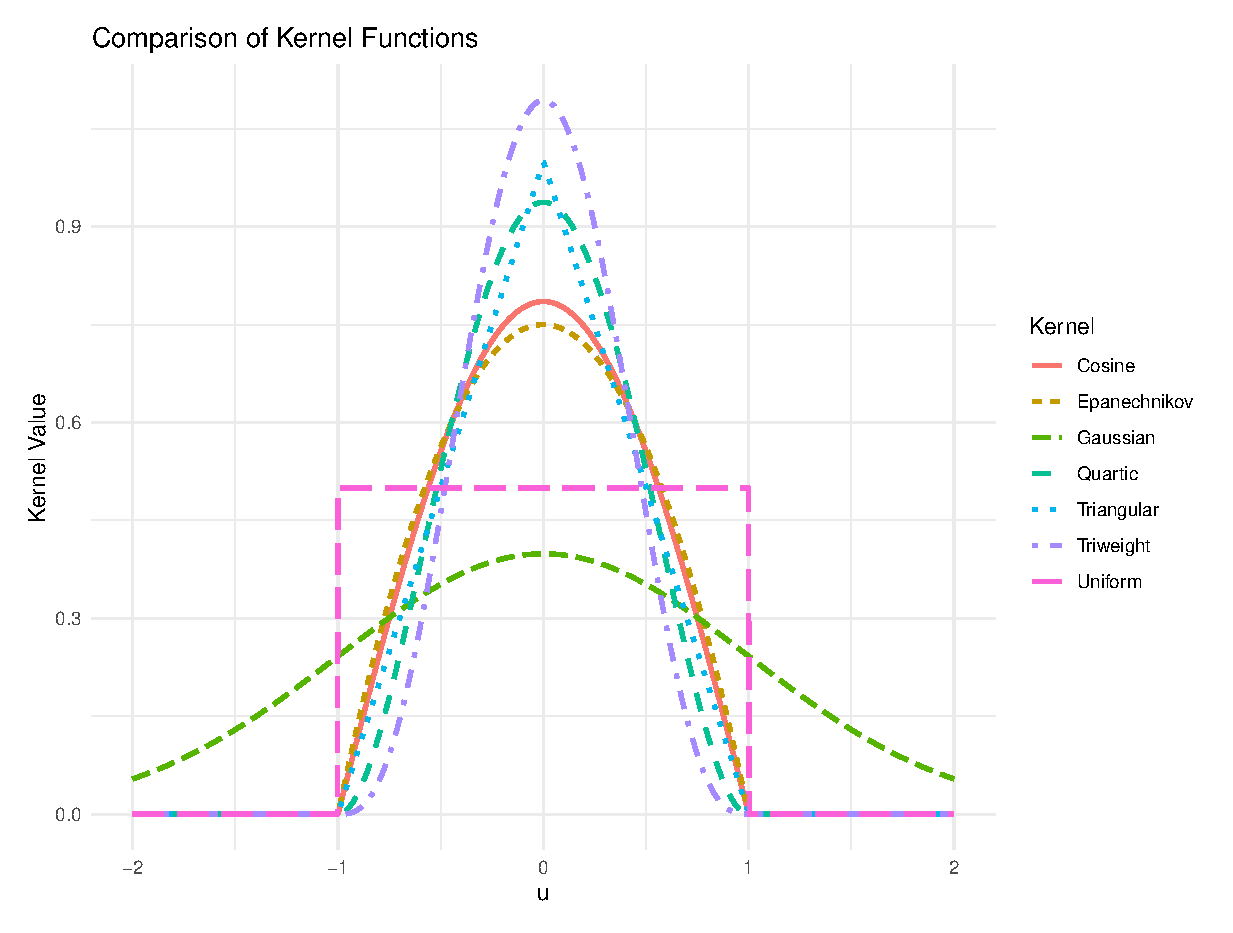
\includegraphics[width=0.9\textwidth,height=0.5\textwidth]{kernel_comparison.eps}
%\end{figure}

\newpage
{\LARGE\centerline{\textbf{Convolutions}\footnote{\cite[Chapter V, Section~4]{fellerv2}.} }}
\vskip25pt
\begin{minipage}{0.9\textwidth}
    \Large 
    Let $\phi$ be a bounded function, $F$ be a probability distribution with density function $f$. The convolution of a function $\phi$ with a probability function $F$ is given by 
    \begin{equation}
        \left(f*\phi\right)(x):=\int_{\R}\phi(x-y)F\{\mathrm{d}y\}=\int_{\R}\phi(x-y)f(y)\mathrm{d}y.
    \end{equation}
    {\bf Claim~1:} If $\phi$ is bounded and continuous, so is $f*\phi$. If $\phi$ is a probability distribution function, so is $f*\phi$.
    \vskip 5pt
    {\bf Claim~2:} Among distributions, the convolution operator is commutative and associative. 
\end{minipage}

\newpage
{\LARGE\centerline{\textbf{A probabilistic interpretation}}}
\vskip25pt
\large
% \begin{minipage}{0.9\textwidth}
\noindent
Suppose the kernel function $K$ is a prob. density function, and $h>0$ small. 
 \vskip 5pt
 \begin{thm}
    The kernel density estimator defined in Eq.\eqref{def-kde} is an unbiased estimator for the density function of random variable $X+hZ$, where $Z$ is an independent random variable with density function $K$.
 \end{thm}
 \begin{proof}
    Because of the independence of $X$ and $Y$, the density function of RV $X+hY$ can be obtained as $f*K_h$.  
    For any $x\in\R$, we have
    \begin{eqnarray}
        \IP(X+hY\le x)&=&\int_{\R}\IP(t+hY\le x)f(t)\mathrm{d}t\nonumber\\
        &=&\int_{\R}\IP\left(Y\le \frac{x-t}h\right)f(t)\mathrm{d}t.
    \end{eqnarray}
    Hence, by taking derivative w.r.t. $x$ in both sides, we have
    \begin{eqnarray*}
        \frac{\mathrm{d}}{\mathrm{d}x}\IP(X+hY\le x)&=&\frac{\mathrm{d}}{\mathrm{d}x}\int_{\R}\IP\left(Y\le \frac{x-t}h\right)f(t)\mathrm{d}t\\
        &=&\int_{\R}\frac{\mathrm{d}}{\mathrm{d}x}\IP\left(Y\le \frac{x-t}h\right)f(t)\mathrm{d}t\\
        % &=&\int_{\R}\frac1hK\left(\frac{x-t}h\right)f(t)\mathrm{d}t\\
        &=&\int_{\R}K_h(x-t)f(t)\mathrm{d}t=\left(K_h*f\right)(x). 
    \end{eqnarray*}
    On the other hand, with Eq.~\eqref{def-kde}, we have 
    \begin{eqnarray}\label{mean-kde}
        \E\left[\hat{f}(x)\right]=\E\left[K_h(x-X_1)\right]=\int_{\R}K_h(x-t)f(t)\mathrm{d}t=\left(K_h*f\right)(x).
    \end{eqnarray}
 \end{proof}
 \noindent
 A direct advantage of this theorem is that the mean function $f*K_h$ of $\hat{f}(x)$ will inherit all the continuity and differentiability properties of $K$.
\begin{rem}
Now, if we take another look at Eq.~\eqref{def-kde}, 
\begin{equation*}
    \hat{f}(x)=\frac1n\sum_{i=1}^nK_h(x-X_i), 
\end{equation*}
the kernel density estimator can be understood as an unbiased density estimator for the data with noise when $h>0$ is small.
\end{rem}
% For our purpose, in the rest of this slides we assume that 
% % {\bf Assumptions:}
%     \begin{enumerate}
%         \item $K$ is a p.d.f.;
%         \item $Z$ is a RV with density $K$, independent with $X$; 
%         \item $\int xK(x)\mathrm{d}x=0$ and $\int x^3 K(x)\mathrm{d}x<\infty$, a.k.a. $\E(Z)=0$ and $\E[Z^3]<\infty$.
%     \end{enumerate}
%     Meanwhile, we also notice it is common in practice that taking $K$ a symmetric p.d.f., see Table~\ref{tabkernels}. However, it seems not an essential assumption. 
\newpage
{\LARGE\centerline{\textbf{R code}}}
\vskip15pt
% \begin{minipage}{.9\textwidth}
    \Large
% R code:  
\begin{enumerate}
\item density()
\begin{Sinput}
density(X, bw="?",  kernel = "?")
# options for bw: a value for bandwidth, or a method:
"nrd0", "nrd", "SJ", "bcv"
    
# options for kernel: "gaussian", "epanechnikov",
"rectangular", "triangular", "biweight", "cosine"
    
\end{Sinput}
\item kde(X, H) where H is the bandwidth, it can be any positive value, but will be discussed later.
\begin{Schunk}
\begin{Sinput}
faithful
# code 1
library(ks)
myout = kde(faithful$eruptions)
hist(faithful$eruptions, freq = FALSE, ylim=c(0, 0.7), 20)
lines(density(faithful$eruptions, kernel = "gaussian",
bw=0.2), col="red")
lines(density(faithful$eruptions, kernel = "gaussian",
bw="SJ"), col="blue")
lines(myout$eval.points, myout$estimate, col="yellow")
# code 2
library(ggplot2)
# Combined histogram and kernel density plot using ggplot2
p <- ggplot(faithful, aes(x = eruptions)) +
geom_histogram(aes(y = after_stat(density)), binwidth = 0.2,
 fill = "lightblue", color = "black") +
geom_density(color = "red", fill = NA) +
labs(title = "Histogram and Kernel Density Plot of Eruptions",
       x = "Eruption Duration (minutes)",
       y = "Density") +
  theme_minimal()
print(p)
\end{Sinput}
\end{Schunk}
% # Save the plot as an EPS file
% # ggsave("faithful_eruptions_hist_density.eps", plot = p, device = "eps", width = 8, height = 6)
\end{enumerate}
\begin{center}
    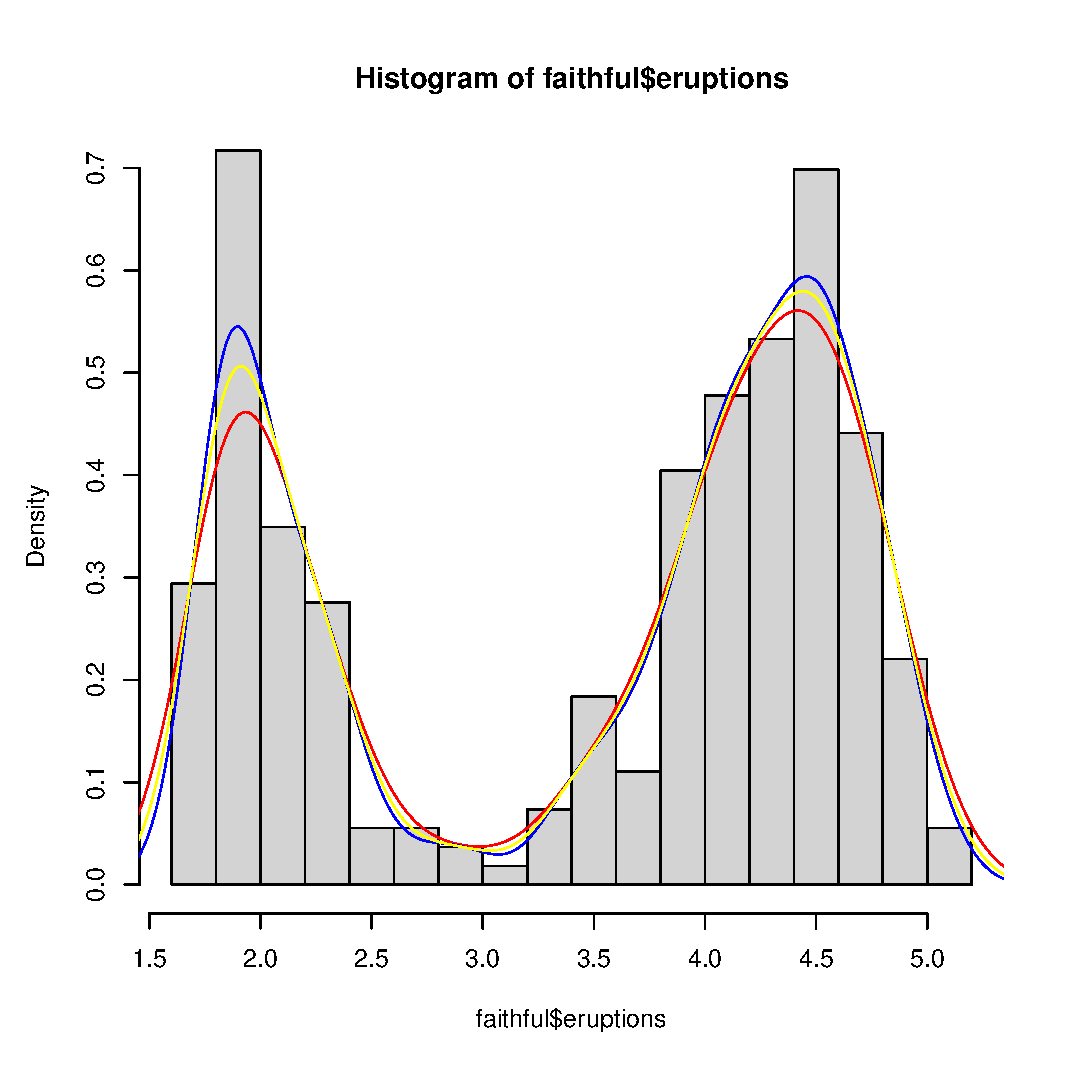
\includegraphics[width=0.9\textwidth,height=0.5\textwidth]{erpt-kernel.eps}
\end{center}
\newpage
{\LARGE\centerline{\textbf{Statistical Properties}}}
\vskip15pt
% \begin{minipage}{.9\textwidth}
    \large \noindent
    For our purpose, in the rest of this slides we assume that 
    \begin{enumerate}
        \item $K$ is a p.d.f.;
        \item $Z$ is a RV with density $K$, independent with $X$; 
        \item $K$ is symmetric, i.e. $K(x)=K(-x)$ for any $x\in\R$;\label{con-symm}
        \item $\int x^3 K(x)\mathrm{d}x=\E(Z^3)<\infty$.
    \end{enumerate}
    We found these assumptions are very common in practice, for example see Table~\ref{tabkernels}. 
    Besides, we also assume that $f''$ is continuous, and the third derivative $f^{(3)}$ of $f$ exists.
% \begin{rem}
%     From one side, Condition~\ref{con-symm} is quite reasonable for $K$ as an smoothing function. On the other hand, it is not necessary to the proofs below. Indeed, it can be replaced by a weaker condition: 
%     \begin{equation}
%         \int_{\R}xK(x)\mathrm{d}x=\E(Z)=0.
%     \end{equation}
% \end{rem}
    \begin{itemize}
        \item Bias: recalling \eqref{mean-kde}, we have 
        \begin{eqnarray}
            \bs\left\{\hat{f}(x)\right\}&=&\E\left[\hat{f}(x)\right]-f(x)\nonumber\\
            &=&(K_h*f)(x)-f(x)\nonumber\\
            &=&\int_{\R}f(x-y)K_h(y)\mathrm{d}y-f(x)\nonumber\\
            &=&\int_{\R}[f(x-y)-f(x)]K_h(y)\mathrm{d}y\nonumber\\
            &=&\int_{\R}\left[(-y)f'(x)+\frac12y^2f''(x)+\frac16y^3f^{(3)}(u^*)\right]K_h(y)\mathrm{d}y\\
            &=&-\E(hZ)f'(x)+\frac12\E[(hZ)^2]f''(x)+o(h^2)\nonumber\\
            &=&\frac{h^2}2\var(Z)f''(x)+o(h^2).\label{bs-est1}
        \end{eqnarray}
        \item Variance:
        \begin{eqnarray}
            \var\left(\hat{f}(x)\right)&=&\frac1n\var\left(K_h(x-X_1)\right)\nonumber\\
            &=&\frac1n\E\left\{[K_h(x-X_1)-(K_h*f)(x)]^2\right\}\nonumber\\
            &=&\frac1n\left\{\E\left[K_h(x-X_1)^2\right]-(K_h*f)(x)^2\right\}.
        \end{eqnarray}
        From \eqref{bs-est1}, we have 
        \begin{equation}\label{boun1}
            (K_h*f)(x)^2=\left[f(x)+O(h^2)\right]^2=f(x)^2+O(h^2).
        \end{equation}
        Furthermore, because $K$ is symmetric, we have 
        \begin{eqnarray}
            \E\left[K_h(x-X_1)^2\right]&=&\int_{\R}K_h(x-y)^2f(y)\mathrm{d}y\nonumber\\
            &=&\frac1{h^2}\int_{\R}K\left(\frac{x-y}h\right)^2f(y)\mathrm{d}y\\
            &=&\frac1{h^2}\int_{\R}K\left(\frac{y-x}h\right)^2f(y)\mathrm{d}y\\
            &=&\frac1{h^2}\int_{\R}K(t)^2f(x+th)h\mathrm{d}t\nonumber\\
            &=&\frac1h\int_{\R}K(t)^2[f(x)+thf'(x)+o(h)]\mathrm{d}t\\
            &=&h^{-1}f(x)\|K\|_{L^2}^2+o(1),\label{boun2}
        \end{eqnarray}
        where $\|g\|_{L^2}^2:=\int_{\R}g(u)\mathrm{d}u$. 
        Combining \eqref{boun1} and \eqref{boun2}, we have 
        \begin{equation}
            \var\left(\hat{f}(x)\right)=\frac1{nh}f(x)\|K\|_{L^2}^2+O(n^{-1}).
        \end{equation}
    \end{itemize}
% \end{minipage}


\newpage
{\LARGE\centerline{\textbf{Continuity condition and MSE}}}
\vskip25pt
\begin{minipage}{.9\textwidth}
    \Large
        For a function $g:\R\to\R$, suppose that for any $x,y\in\R$, it holds 
        \begin{equation}
            |g(x)-g(y)|\le K|x-y|^\alpha,
        \end{equation}
        for some $\alpha>0$. 
        For $\alpha=1$, such functions are called {\it Lipschitz functions}. For $0<\alpha<1$, they are said to satisfy a {\it H\"older condition} of order $\alpha$, c.f.\cite[Page~56]{Dudley02}. 
\vskip 5pt
        For a function $g$ defined on a finite interval $[a,b]$ with $a<b$, 
        $$\mathrm{Lipschitz~continous}\Rightarrow \mathrm{H\ddot{o}lder~continuous}\Rightarrow \mathrm{uniformly~continuous}.$$
Mean Square Error (MSE) of $\widehat{f}_h(x)$, defined by 
\begin{eqnarray}
    {\rm MSE}\left(\widehat{f}_h(x)\right):=\E\left[\left|\widehat{f}_h(x)-f(x)\right|^2\right],
\end{eqnarray}
is a widely used performance measure of an estimator. 
\end{minipage}

\newpage
{\LARGE\centerline{\textbf{Main Theorem}}}
\vskip25pt
\begin{minipage}{.9\textwidth}
    \large
\begin{thm}\label{thm1-L2}
    Suppose the density function $f$ is Lipschitz continuous on the interval $B_j$. When $n^{-1}\ll h\ll1$, the histogram $\widehat{f}_h(x)$ converges to $f(x)$, in the mean square sense,  i.e. 
    \begin{equation}
        {\rm MSE}\left\{\widehat{f}_h(x)\right\}\to0,
    \end{equation}
    as $n\to\infty$.
\end{thm}
\begin{proof}
    Since $f$ is Lipschitz continuous on $B_j$, from \eqref{bs-mvt}, we have
    \begin{equation}\label{bs-bound}
        \left|\bs\left\{\widehat{f}_h(x)\right\}\right|=\left|f(u^*)-f(x)\right|\le K|u^*-x|\le Kh.
    \end{equation}
    Furthermore, from \eqref{var-bound1}, we have 
    \begin{equation}\label{var-bound2}
        \var\left(\widehat{f}_h(x)\right)\le C(nh)^{-1}
    \end{equation} for some constant $C$, 
    as $f$ is bounded on $B_j$, implied by the Lipschitz continuity. Combining \eqref{bs-bound} with \eqref{var-bound2}, we have
    \begin{equation} \label{bound-mse1}
        {\rm MSE}\left\{\widehat{f}_h(x)\right\} =\left(\bs\left\{\widehat{f}_h(x)\right\}\right)^2+\var\left(\widehat{f}_h(x)\right)\le K^2h^2+C(nh)^{-1}\to0.
    \end{equation}
\end{proof}
{\small An easy trick: $E(X-a)^2=\E(X-\E(X)+\E(X)-a)^2=\Var(X)+(\E(X)-a)^2$.}
\end{minipage}

\newpage
{\LARGE\centerline{\textbf{Selection of binwidth}}}
\vskip25pt
\begin{minipage}{.9\textwidth}
    \Large The binwidth $h$ is referred to be a {\it smoothing parameter} in the literature on smoothing. 

    The inequality in \eqref{bound-mse1} summarizes the trade-off between bias and variance is determined by the choice of smoothing parameter. 

    We can take the upper bound in \eqref{bound-mse1} as a function of $h$, and achieve its minimal point at $h_{\min}:=[C(2nK^2)^{-1}]^{1/3}$. 
    
    Plugging $h_{\min}$ in \eqref{bound-mse1}, we have
    $${\rm MSE}\left\{\widehat{f}_h(x)\right\}=O\left(n^{-2/3}\right).$$
    Note, if we assume $f$ satisfying H\"older condition of order $\alpha$, for some $0<\alpha<1$, instead of Lipschitz continuity in Theorem~\ref{thm1-L2}, we can obtain 
    $${\rm MSE}\left\{\widehat{f}_h(x)\right\}=O\left(n^{-\frac{2\alpha}{2\alpha+1}}\right).$$
\end{minipage}

\newpage
{\LARGE\centerline{\textbf{Bin number selection}}}
\vskip25pt
\begin{minipage}{.9\textwidth}
    \Large 
\begin{itemize}
    \item Sturges' rule, c.f. \cite{sturges26};
    \item Doane's formula, c.f. \cite{doane76};
    \item Scott's rule, c.f. \cite{scott79};
    \item Freedman-Diaconis rule, c.f. \cite{FreedmanDiaconis81}. 
\end{itemize}
\end{minipage}

\newpage
{\LARGE{\textbf{Sturges' rule}}}
\vskip25pt
\begin{minipage}{.9\textwidth}
    \Large 
{\it Sturges' rule} is a method of selecting the number of bins for a histogram, being widely employed in statistical and data analysis software, including Python and R. 

Originating from the idea that using (symmetric) binomial distribution to approximate discretized normal distribution, \cite{sturges26} considers an idealized histogram with $k$ bins, where the $i$-th bin count is binomial coefficient ${k-1 \choose i}$, for $i=0,1,\dots,k-1$. As $k$ increase, this ideal histogram approaches the shape of a normal density. 

The total sample size is 
$$n=\sum_{i=0}^{k-1}{k-1 \choose i}=(1+1)^{k-1}=2^{k-1},$$
by the binomial formula. Sturges' rule for number of bins follows immediately:
\begin{equation}\label{sturges-rule}
    k=1+\log_2n.
\end{equation}
\end{minipage}

\newpage
{\LARGE{\textbf{Doane's rule}}}
\vskip15pt
\begin{minipage}{.9\textwidth}
    \Large 
If the data are not normal distributed, but are skewed, additional bins may be necessary. \cite{doane76} proposes increases the number of bins in \eqref{sturges-rule} by 
\begin{equation}\label{doane-rule}    k=\log_2(1+\hat{\gamma}_3\sqrt{n/6}),
\end{equation}
where 
$$\hat{\gamma}_3=\frac{n^{-1}\sum_{i=1}^n(x_i-\bar{x})^3}{(n^{-1}\sum_{i=1}^n(x_i-\bar{x})^2)^{3/2}}$$
is an estimate of the standardized skewness coefficient. 
\end{minipage}

\newpage
{\LARGE{\textbf{Mean Integrated Squared Error}}}
\vskip15pt
\begin{minipage}{.9\textwidth}
    \Large 
Instead of focusing on the accuracy of $\widehat{f}_h(x)$ as an estimator of $f$ at one single point, people are more likely to be interested in a global measure of accuracy. The most widely used global measure of estimation accuracy is the {\it mean integrated squared error} (MISE), 
\begin{eqnarray}
    {\rm MISE}\{\widehat{f}_h\}&:=&\E\left[\int_{\R}\left(\widehat{f}_h(x)-f(x)\right)^2\mathrm{d}x\right]\\
&=&\int_{\R}\E\left[\left(\widehat{f}_h(x)-f(x)\right)^2\right]\mathrm{d}x\nonumber\\
&=&\int_{\R}{\rm MSE}\{\widehat{f}_h(x)\}\mathrm{d}x.
\end{eqnarray}

\end{minipage}

\newpage
{\LARGE{\textbf{Mean Integrated Squared Error (cont.)}}}
\vskip15pt
\begin{minipage}{.9\textwidth}
    \Large 
    With stronger assumptions on the derivative $f'$, the asymptotic MISE is\footnote{See \cite[Section~3.2]{scott15} for more detailed analysis.}
    $${\rm AMISE}(h)=\frac1{nh}+\frac1{12}h^2\|f'\|_2^2.$$
    Hence, as we did for \eqref{bound-mse1}, minimizing at $h^*=\left[\frac6{n\|f'\|_2^2}\right]^{1/3}$, 
    \begin{equation}
    {\rm AMISE}(h^*)=(3\|f'\|_2/4)^{2/3}n^{-2/3}.
    \end{equation}
    Taking the density of normal distribution $\mathcal{N}(\mu,\sigma^2)$ as a reference, $\|f'\|_2^2=(4\sqrt{\pi}\sigma)^{-1}$
    \begin{equation}
        h^*=(24\sqrt{\pi})^{1/3}\sigma n^{-1/3}\approx 3.5\sigma n^{-1/3}.
        \end{equation}
        \begin{itemize}
            \item Scott's rule: $\hat{h}=3.5\hat{\sigma}n^{-1/3}$;
            \item Freedman-Diaconis's rule: $\hat{h}=2({\rm IQR})n^{-1/3},$ where ${\rm IQR}$ is the interquartile range. 
        \end{itemize}
\end{minipage}

\newpage
{\LARGE\centerline{\textbf{Summary}}}
\vskip25pt
\begin{minipage}{.9\textwidth}
    \Large 
    The optimal $O(n^{-2/3})$ for AMISE is unsatisfactorily slow, as \cite{boydsteele78} shows the best possible rate is $O(n^{-1})$ in the parametric approach. This deficiency can be regarded as the price for generality, i.e. removing parametric assumptions.  

    % \begin{Sinput}
    %     library(ggplot2)
    %     home_data <- read.csv("https://raw.github
    %     usercontent.com/rashida048/Datasets/mast
    %     er/home_data.csv")[ ,c('price', 'condition')]
    % \end{Sinput}
    \vskip 10pt
    {\huge Using chatGPT!}
\end{minipage}


% \newpage
% {\LARGE{\textbf{Histogram in R}}}
% \vskip25pt

% \begin{figure}[h]
% \centering
%       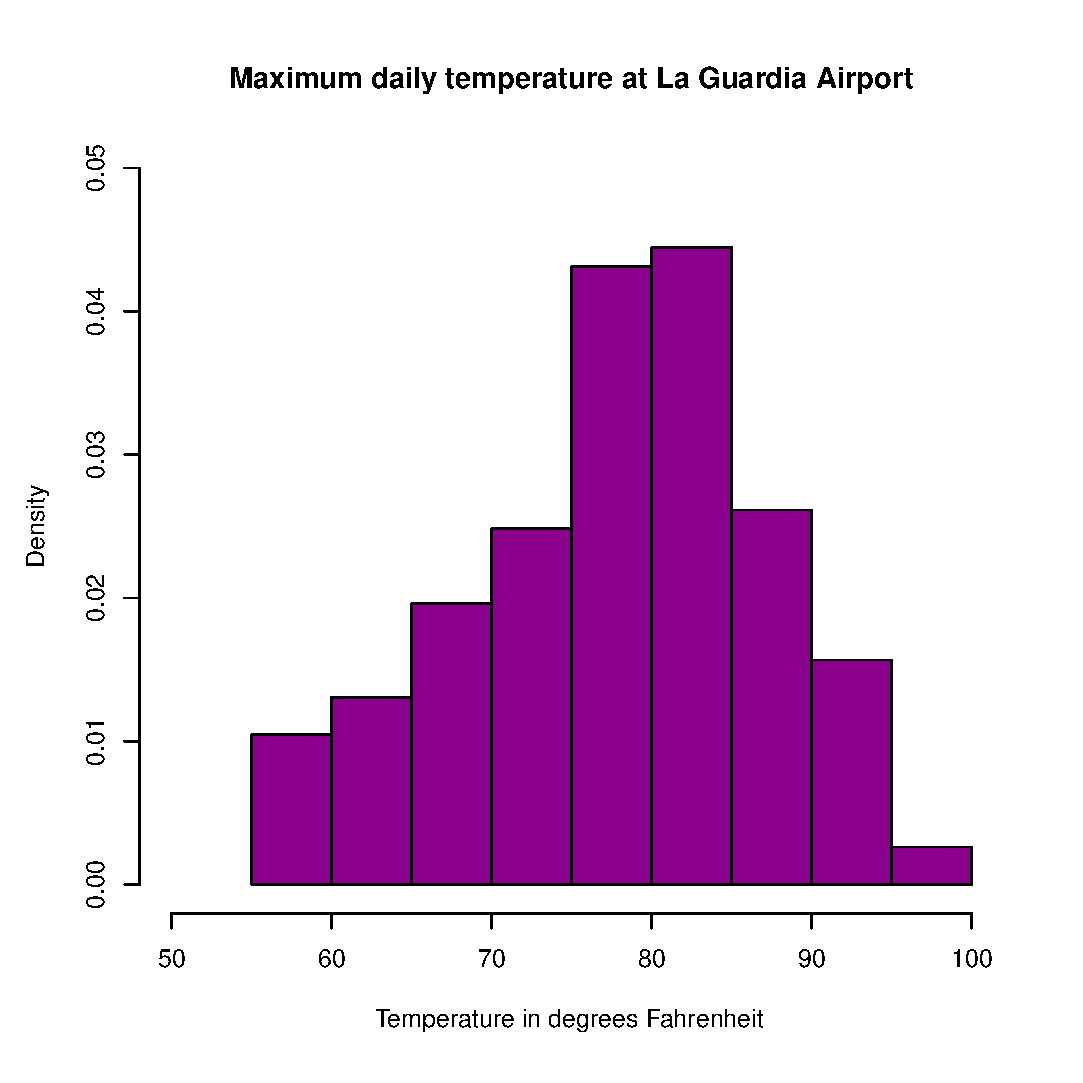
\includegraphics[width=0.75\textwidth,height=0.52\textwidth]{temperature.eps}
%     \label{figure5} 
% \end{figure}
% (Data source: built-in dataset airquality which has "Daily air quality measurements in New York, May to September 1973" -R documentation.)
% \newpage
% {\LARGE{\textbf{Histogram of house prices using Sturges' Rule}}}
% \vskip25pt

% \begin{figure}[h]
% \centering
%       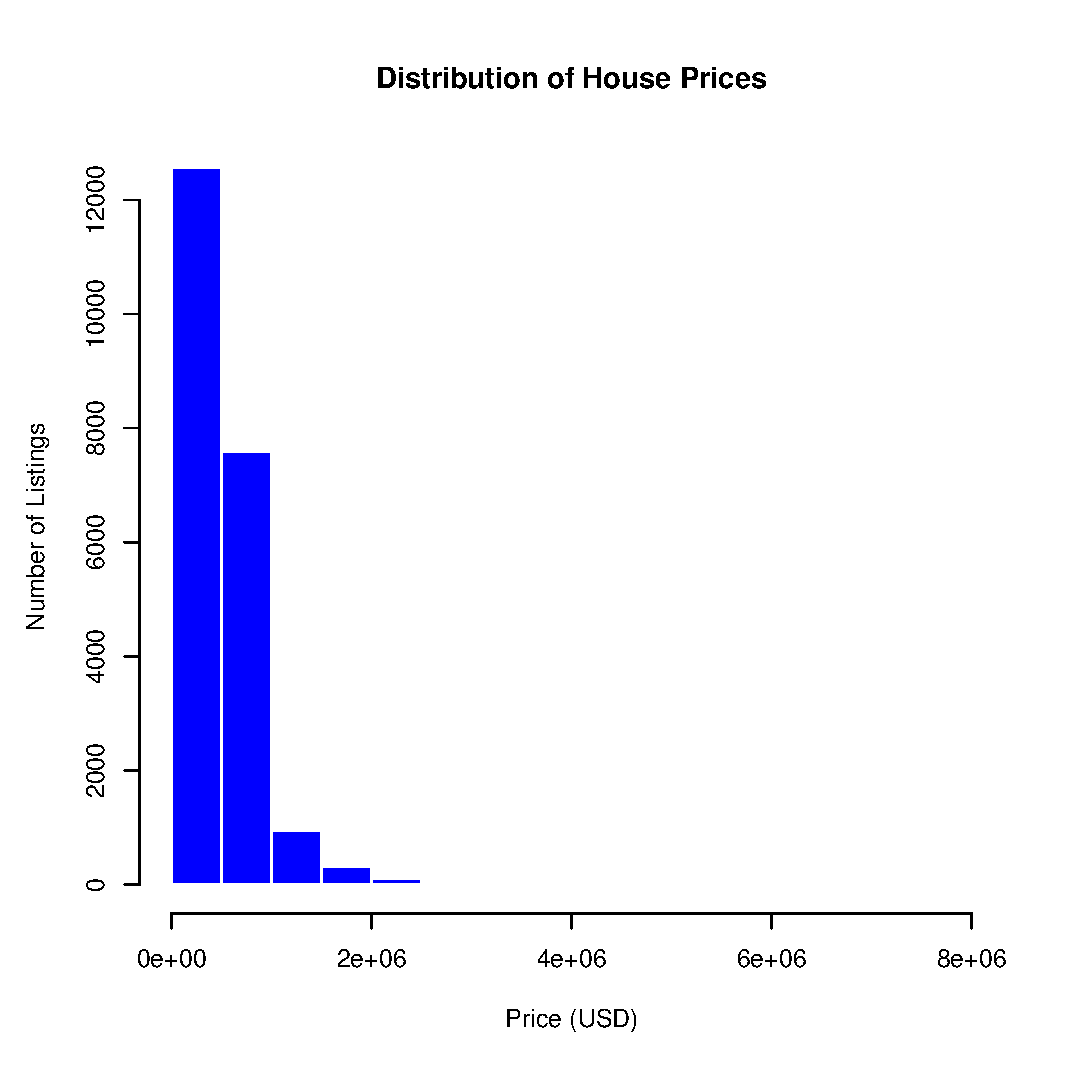
\includegraphics[width=0.75\textwidth,height=0.52\textwidth]{hist_housing_default.eps}
%     \label{figure6} 
% \end{figure}
% (Data source: \href{https://raw.githubusercontent.com/rashida048/Datasets/master/home_data.csv}{House Data}, \textcolor{red}{breaks = "Sturges"})

% \newpage
% {\LARGE{\textbf{Histogram of house prices using Scott's Rule}}}
% \vskip25pt

% \begin{figure}[h]
% \centering
%       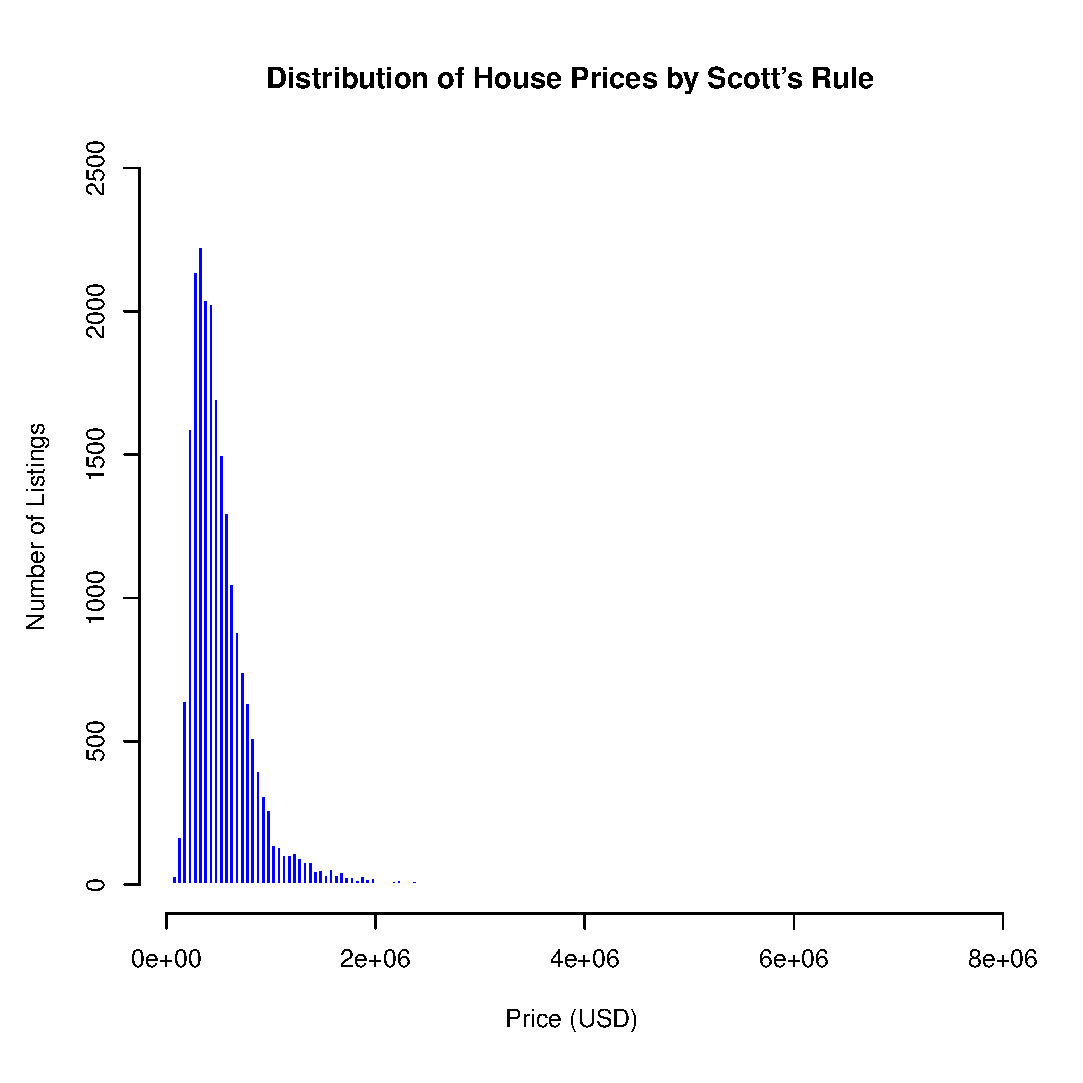
\includegraphics[width=0.75\textwidth,height=0.52\textwidth]{hist_housing_Scott.eps}
%     \label{6} 
% \end{figure}
% (Data source: \href{https://raw.githubusercontent.com/rashida048/Datasets/master/home_data.csv}{House Data}, \textcolor{red}{breaks = "Scott"})

% \newpage
% {\LARGE{\textbf{Histogram of house prices using Freedman-Diaconis's Rule}}}
% \vskip25pt

% \begin{figure}[h]
% \centering
%       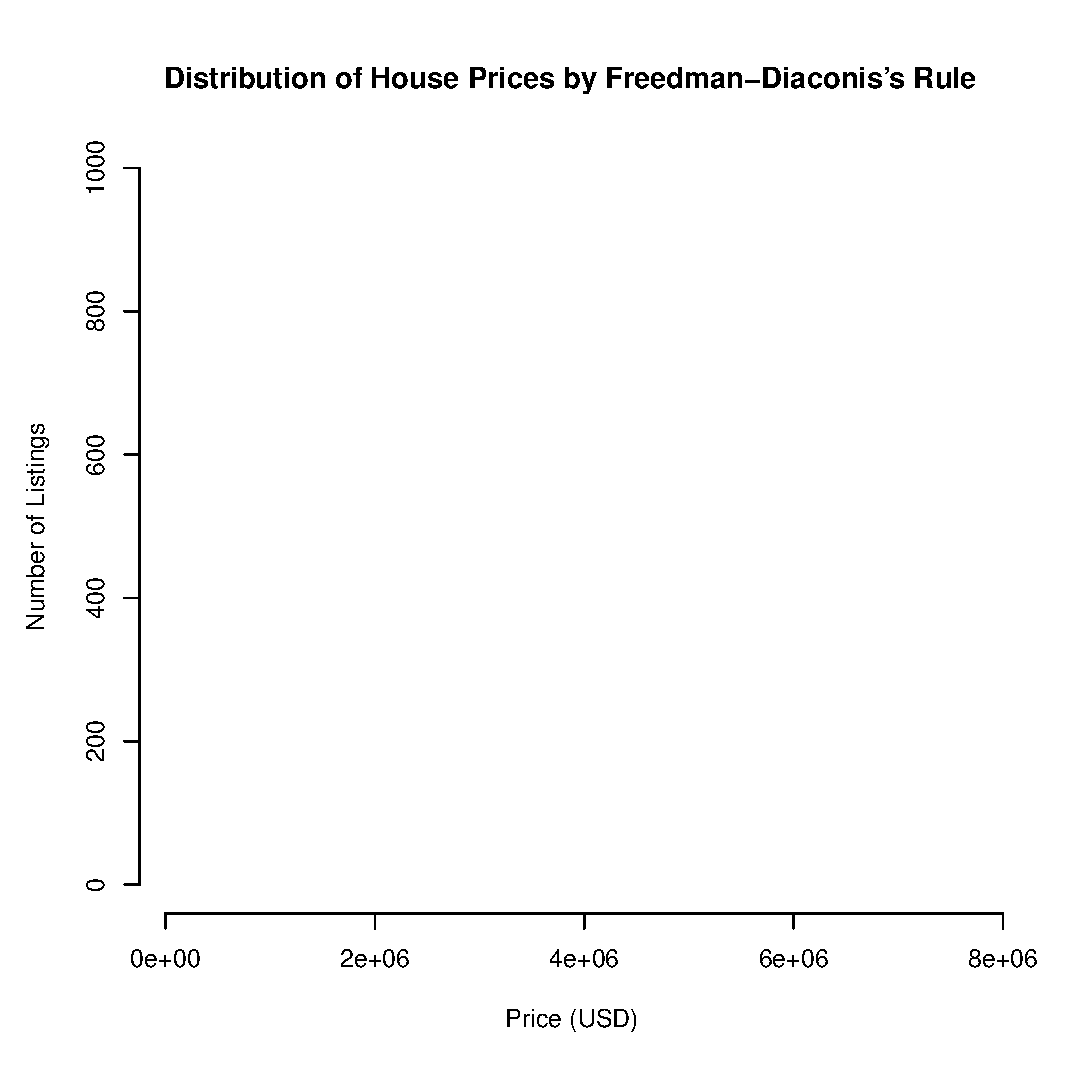
\includegraphics[width=0.75\textwidth,height=0.52\textwidth]{hist_housing_Freedman.eps}
%     \label{figure7} 
% \end{figure}
% (Data source: \href{https://raw.githubusercontent.com/rashida048/Datasets/master/home_data.csv}{House Data}, \textcolor{red}{breaks = "Freedman-Diaconis"})

\newpage
{\LARGE\centerline{\textbf{Consistency}}}
\vskip25pt
\begin{minipage}{.9\textwidth}
    \Large 
\begin{defi}[\cite{garthwaite02}]
    An estimator $\hat{\theta}$ for $\theta$ is (weakly) consistent if $\IP(|\hat{\theta}-\theta|>\epsilon)\to0$ as $n\to\infty$ for any $epsilon>0$, i.e. $\hat{\theta}$ converges to $\theta$ in probability.
\end{defi} 
{\bf Claim:} ${\rm MSE}\{\hat{\theta}\}\to0$ implies consistency. 
\begin{eqnarray*}
    \IP(|\hat{\theta}-\theta|>\epsilon)=\E\left[\bone_{\{|\hat{\theta}-\theta|>\epsilon\}}\right]&\le&\E\left[\frac{|\hat{\theta}-\theta|^2}{\epsilon^2}\bone_{\{|\hat{\theta}-\theta|>\epsilon\}}\right]\\
    &\le&\epsilon^{-2}\E\left[|\hat{\theta}-\theta|^2\right].
\end{eqnarray*}
\end{minipage}

\newpage
{\LARGE\centerline{\textbf{Cumulants}}}
\vskip25pt
\begin{minipage}{.9\textwidth}
    \large 
  \begin{itemize}
    \item[$\blacktriangleright$] Moments and moment generating function (MGF)
    \begin{equation*}
        \E\left(e^{tX}\right)=\sum_{n\ge0}\frac{t^n}{n!}\E(X^n).
    \end{equation*}
    \item[$\blacktriangleright$] $\log$-MGF: Cumulants and their generating function
\begin{equation*}
    \log\E\left(e^{tX}\right)=\sum_{n\ge0}\frac{t^n}{n!}\kappa_n(X).
\end{equation*}
    \item[$\blacktriangleright$] Cumulants to moments:
\begin{eqnarray}
    \kappa_1(X)&=&\E(X),\nonumber\\
    \kappa_2(X)&=&\E[(X-\E[X])^2],\nonumber\\
    \kappa_3(X)&=&\E[(X-\E[X])^3],\nonumber\\
    \kappa_4(X)&=&\E[(X-\E[X])^4]-3(\E[(X-\E[X])^2])^2.\nonumber
\end{eqnarray}
    \item[$\blacktriangleright$] Skewness  $\kappa_3/\kappa_2^{3/2}$, and 
  \end{itemize}
\end{minipage}

\newpage
{\LARGE\centerline{\textbf{Landau's symbol}}}
\vskip25pt
\begin{minipage}{.9\textwidth}
   \Large
   We also recall the following standard notation for the asymptotic behavior of the relative order of magnitude of two functions $f(n)$ and $g(n )>0$ as $n$ tends to infinity.
   We write
   \begin{itemize}
      \item
        $f(n)=O(g(n))$,
        or $f(n ) \lesssim g(n )$, if $\limsup_{n \to\infty} f(n ) / g(n ) <\infty$;
      \item
        $f(n)=\Omega(g(n ))$, or 
        $f(n ) \gtrsim g(n )$, if $\liminf_{n \to\infty} f(n) / g(n)>0$;
    % \item       $f(\lambda )=\Theta(g(\lambda ))$ if $f(\lambda )=O(g(\lambda ))$ and $f(\lambda )=\Omega(g(\lambda ))$, 
      \item $f(n)\asymp g(n)$ if $f(n)=O(g(n))$ and $f(n)=\Omega(g(n))$; % if $f(\lambda )=\Theta(g(\lambda ))$;
  % \item $f(\lambda )\sim g(\lambda )$ if $\lim_{\lambda \to \infty} f(\lambda )/g(\lambda ) = 1$, 
     \item $f(n)=o(g(n))$, if $f(n)/g(n)\to 0$;
  %    \item $f(x)\ll g(x)$, or $g(x)\gg f(x)$ if $f(x)\ge0$ and $f(x)=o(g(x))$.
      \item $f(n)\ll g(n)$, or $g(n)\gg f(n)$, if $f(n)\ge0$ and $f(n)/g(n)\to 0$.
  \end{itemize}
  Find more details in this Wikipedia page of \href{https://en.wikipedia.org/wiki/Big_O_notation#History_(Bachmann–Landau,_Hardy,_and_Vinogradov_notations)}{Big O notation}.
\end{minipage}







\newpage
\bibliographystyle{apalike}
\bibliography{../ref}
% \begin{thebibliography}{}

%     \bibitem[Boyd and Steele, 1978]{boydsteele78}
%     Boyd, D.~W. and Steele, J.~M. (1978).
%     \newblock Lower bounds for nonparametric density estimation rates.
%     \newblock {\em Ann. Statist.}, 6(4):932--934.
    
%     \bibitem[Doane, 1976]{doane76}
%     Doane, D.~P. (1976).
%     \newblock Aesthetic frequency classifications.
%     \newblock {\em Amer. Statist.}, 30(4):181--183.
    
%     \bibitem[Dudley, 2002]{Dudley02}
%     Dudley, R.~M. (2002).
%     \newblock {\em Real Analysis and Probability}.
%     \newblock Cambridge Studies in Advanced Mathematics. Cambridge University Press, Cambridge, 2 edition.
    
%     \bibitem[Freedman and Diaconis, 1981]{FreedmanDiaconis81}
%     Freedman, D. and Diaconis, P. (1981).
%     \newblock On the histogram as a density estimator: $L_2$ theory.
%     \newblock {\em Probab. Theory Related Fields}, 57(4):453--476.
    
%     \bibitem[Garthwaite et~al., 2002]{garthwaite02}
%     Garthwaite, P.~H., Jolliffe, I.~T., and Jones, B. (2002).
%     \newblock {\em Statistical inference}.
%     \newblock OUP Oxford.
    
%     \bibitem[Scott, 1979]{scott79}
%     Scott, D.~W. (1979).
%     \newblock {On optimal and data-based histograms}.
%     \newblock {\em Biometrika}, 66(3):605--610.
    
%     \bibitem[Scott, 2015]{scott15}
%     Scott, D.~W. (2015).
%     \newblock {\em Multivariate density estimation: theory, practice, and visualization}.
%     \newblock Wiley Series in Probability and Statistics. John Wiley \& Sons, 2nd edition.
    
%     \bibitem[Sturges, 1926]{sturges26}
%     Sturges, H.~A. (1926).
%     \newblock The choice of a class interval.
%     \newblock {\em J. Amer. Statist. Assoc.}, 21(153):65--66.
    
%     \end{thebibliography}
    
\end{document}